\section{Native ANSYS from first exposure to burnthrough}\label{sec:whole}
The liner and casing start at 22~$^\circ$C. From first exposure to liner loss,
the model holds the gas at 2504~K and 800~psi with a nominal film coefficient of
1000~W/(m$^2$~K). After each MAPDL thermal solve the controller updates
chemistry, surface position and casing state.

\begin{center}\small\begin{tabular}{lrrrrrr}\toprule
 & Casing & Liner left & ANSYS & Radial & Difference & Interval\\
Motor & event [s] & [mm] & gone [s] & gone [s] & [s] & gap [s]\\\midrule
Sustainer Al & 99.14 & 0.430 & 110.58 & 110.47 & +0.102 & 0.066 \\
Sustainer CF & 95.16 & 0.453 & 104.33 & 104.25 & +0.078 & 0.042 \\
Booster Al & 139.44 & 0.229 & 147.75 & 147.61 & +0.136 & 0.100 \\
\bottomrule\end{tabular}\end{center}
The casing event marks complete Al fusion or the CF reaching 1000~$^\circ$C.
The liner thickness there is interpolated between half-second samples. Times
use the upper ends of the exhaustion intervals. The gap separates their nearest
ends. Beyond the casing event, the thermal model holds the molten Al or CF
residue in place. Casing pressure capacity remains undetermined.

\begin{figure}[H]\centering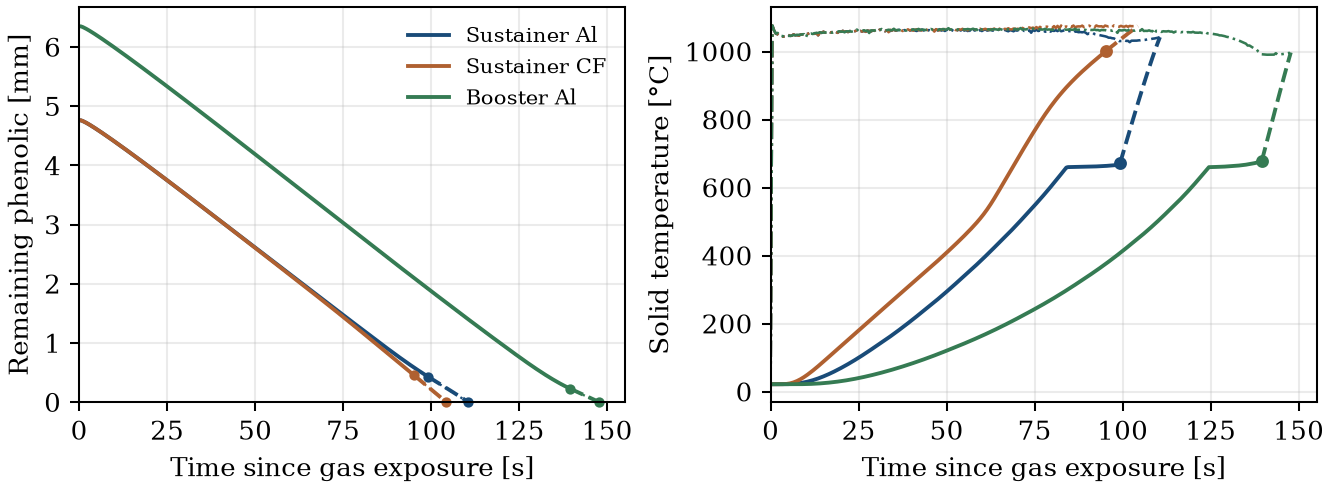
\includegraphics[width=.98\textwidth]{../analysis/native_whole_exposure.png}
\caption{Left, native liner thickness and independent finite-volume
thickness (dotted). Right, native interface and exposed liner (dash-dot)
temperatures. The final surface point precedes liner loss. Dashed lines use the
retained casing model after complete fusion or the CF property limit.}
\end{figure}
\begin{center}\small\begin{tabular}{lrrrrl}\toprule
& Native field & Max.\ thickness & Film dose & Peak live & Time and\\
Motor & solves & diff.\ [$\mu$m] & [MJ/m$^2$] & face [$^\circ$C] & thickness\\\midrule
Sustainer Al & 2,903 & 4.03 & 131.91 & 1076 & Pass \\
Sustainer CF & 2,713 & 3.86 & 122.86 & 1077 & Pass \\
Booster Al & 3,883 & 4.33 & 174.82 & 1076 & Pass \\
\bottomrule\end{tabular}\end{center}
Thickness differences use common half-second samples while liner remains.
Film dose is heat entering the moving wall per original exposed area. A pass
requires event times within 1\% and thickness within the larger of 0.02~mm and
1\% of initial thickness. Both solvers use the same heating and char law.

Replaying all native fields with the sealed controller and an independent
radial thermal system gave a maximum discrepancy of $2.0\times10^{-9}$~K. The largest
absolute energy imbalance was $8.1\times10^{-10}$ of the film dose.
\clearpage
